%% abtex2-modelo-projeto-pesquisa.tex, v-1.9.6 laurocesar
%% Copyright 2012-2016 by abnTeX2 group at http://www.abntex.net.br/ 
%%
%% This work may be distributed and/or modified under the
%% conditions of the LaTeX Project Public License, either version 1.3
%% of this license or (at your option) any later version.
%% The latest version of this license is in
%%   http://www.latex-project.org/lppl.txt
%% and version 1.3 or later is part of all distributions of LaTeX
%% version 2005/12/01 or later.
%%
%% This work has the LPPL maintenance status `maintained'.
%% 
%% The Current Maintainer of this work is the abnTeX2 team, led
%% by Lauro César Araujo. Further information are available on 
%% http://www.abntex.net.br/
%%
%% This work consists of the files abntex2-modelo-projeto-pesquisa.tex
%% and abntex2-modelo-references.bib
%%

% ------------------------------------------------------------------------
% ------------------------------------------------------------------------
% abnTeX2: Modelo de Projeto de pesquisa em conformidade com 
% ABNT NBR 15287:2011 Informação e documentação - Projeto de pesquisa -
% Apresentação 
% ------------------------------------------------------------------------ 
% ------------------------------------------------------------------------

\documentclass[
	% -- opções da classe memoir --
	12pt,				% tamanho da fonte
	openright,			% capítulos começam em pág ímpar (insere página vazia caso preciso)
	twoside,			% para impressão em recto e verso. Oposto a oneside
	a4paper,			% tamanho do papel. 
	% -- opções da classe abntex2 --
	%chapter=TITLE,		% títulos de capítulos convertidos em letras maiúsculas
	%section=TITLE,		% títulos de seções convertidos em letras maiúsculas
	%subsection=TITLE,	% títulos de subseções convertidos em letras maiúsculas
	%subsubsection=TITLE,% títulos de subsubseções convertidos em letras maiúsculas
	% -- opções do pacote babel --
	english,			% idioma adicional para hifenização
	french,				% idioma adicional para hifenização
	spanish,			% idioma adicional para hifenização
	brazil,				% o último idioma é o principal do documento
	]{abntex2}

% ---
% PACOTES
% ---

% ---
% Pacotes fundamentais 
% ---
\usepackage{lmodern}			% Usa a fonte Latin Modern
\usepackage[T1]{fontenc}		% Selecao de codigos de fonte.
\usepackage[utf8]{inputenc}		% Codificacao do documento (conversão automática dos acentos)
\usepackage{indentfirst}		% Indenta o primeiro parágrafo de cada seção.
\usepackage{color}				% Controle das cores
\usepackage{graphicx}			% Inclusão de gráficos
\usepackage{microtype} 			% para melhorias de justificação
% ---

% ---
% Pacotes adicionais, usados apenas no âmbito do Modelo Canônico do abnteX2
% ---
\usepackage{lipsum}				% para geração de dummy text
% ---

% ---
% Pacotes de citações
% ---
\usepackage[brazilian,hyperpageref]{backref}	 % Paginas com as citações na bibl
\usepackage[alf]{abntex2cite}	% Citações padrão ABNT

% --- 
% CONFIGURAÇÕES DE PACOTES
% --- 

% ---
% Configurações do pacote backref
% Usado sem a opção hyperpageref de backref
\renewcommand{\backrefpagesname}{Citado na(s) página(s):~}
% Texto padrão antes do número das páginas
\renewcommand{\backref}{}
% Define os textos da citação
\renewcommand*{\backrefalt}[4]{
	\ifcase #1 %
		Nenhuma citação no texto.%
	\or
		Citado na página #2.%
	\else
		Citado #1 vezes nas páginas #2.%
	\fi}%
% ---

% ---
% Informações de dados para CAPA e FOLHA DE ROSTO
% ---
\titulo{Uso do ambiente R para análise, tratamento e apresentação em tempo real de dados coletados por um Arduíno.}
\autor{Ricardo Aparecido Bezerra Elias da Silva}
\local{Brasil}
\data{2018}
\instituicao{%
  Centro Universitário UNIFIEO
  \par
  Engenharia da Computação
  \par
  Projeto de Iniciação Científica}
\tipotrabalho{Tese (Doutorado)}
% O preambulo deve conter o tipo do trabalho, o objetivo, 
% o nome da instituição e a área de concentração 
\preambulo{Modelo canônico de Projeto de pesquisa em conformidade
com as normas ABNT apresentado à comunidade de usuários \LaTeX.}
% ---

% ---
% Configurações de aparência do PDF final

% alterando o aspecto da cor azul
\definecolor{blue}{RGB}{41,5,195}

% informações do PDF
\makeatletter
\hypersetup{
     	%pagebackref=true,
		pdftitle={\@title}, 
		pdfauthor={\@author},
    	pdfsubject={\imprimirpreambulo},
	    pdfcreator={LaTeX with abnTeX2},
		pdfkeywords={abnt}{latex}{abntex}{abntex2}{projeto de pesquisa}, 
		colorlinks=true,       		% false: boxed links; true: colored links
    	linkcolor=blue,          	% color of internal links
    	citecolor=blue,        		% color of links to bibliography
    	filecolor=magenta,      		% color of file links
		urlcolor=blue,
		bookmarksdepth=4
}
\makeatother
% --- 

% --- 
% Espaçamentos entre linhas e parágrafos 
% --- 

% O tamanho do parágrafo é dado por:
\setlength{\parindent}{1.3cm}

% Controle do espaçamento entre um parágrafo e outro:
\setlength{\parskip}{0.2cm}  % tente também \onelineskip

% ---
% compila o indice
% ---
\makeindex
% ---

% ----
% Início do documento
% ----
\begin{document}

% Seleciona o idioma do documento (conforme pacotes do babel)
%\selectlanguage{english}
\selectlanguage{brazil}

% Retira espaço extra obsoleto entre as frases.
\frenchspacing 

% ----------------------------------------------------------
% ELEMENTOS PRÉ-TEXTUAIS
% ----------------------------------------------------------
% \pretextual

% ---
% Capa
% ---
\imprimircapa
% ---

% ---
% Folha de rosto
% ---
%\imprimirfolhaderosto
% ---

% ---
% NOTA DA ABNT NBR 15287:2011, p. 4:
%  ``Se exigido pela entidade, apresentar os dados curriculares do autor em
%     folha ou página distinta após a folha de rosto.''
% ---

% ---
% inserir lista de ilustrações
% ---
\pdfbookmark[0]{\listfigurename}{lof}
\listoffigures*
\cleardoublepage
% ---

% ---
% inserir lista de tabelas
% ---
\pdfbookmark[0]{\listtablename}{lot}
\listoftables*
\cleardoublepage
% ---

% ---
% inserir lista de abreviaturas e siglas
% ---
%\begin{siglas}
%  \item[ABNT] Associação Brasileira de Normas Técnicas
%  \item[abnTeX] ABsurdas Normas para TeX
%\end{siglas}
% ---

% ---
% inserir lista de símbolos
% ---
%\begin{simbolos}
%  \item[$ \Gamma $] Letra grega Gama
%  \item[$ \Lambda $] Lambda
%  \item[$ \zeta $] Letra grega minúscula zeta
%  \item[$ \in $] Pertence
%\end{simbolos}
% ---

% ---
% inserir o sumario
% ---
\pdfbookmark[0]{\contentsname}{toc}
\tableofcontents*
\cleardoublepage
% ---


% ----------------------------------------------------------
% ELEMENTOS TEXTUAIS
% ----------------------------------------------------------
\textual

% ----------------------------------------------------------
% Introdução
% ----------------------------------------------------------
\chapter*[Introdução]{Introdução}
\addcontentsline{toc}{chapter}{Introdução}

Este documento e seu código-fonte são exemplos de referência de uso da classe
\textsf{abntex2} e do pacote \textsf{abntex2cite}. O documento 
exemplifica a elaboração de projetos de pesquisa produzidos
conforme a ABNT NBR 15287:2011 \emph{Informação e documentação - Projeto de
pesquisa - Apresentação}. 

A expressão ``Modelo canônico'' é utilizada para indicar que \abnTeX\ não é
modelo específico de nenhuma universidade ou instituição, mas que implementa tão
somente os requisitos das normas da ABNT. Uma lista completa das normas
observadas pelo \abnTeX\ é apresentada em \citeonline{abntex2classe}.

Sinta-se convidado a participar do projeto \abnTeX! Acesse o site do projeto em
\url{http://www.abntex.net.br/}. Também fique livre para conhecer,
estudar, alterar e redistribuir o trabalho do \abnTeX, desde que os arquivos
modificados tenham seus nomes alterados e que os créditos sejam dados aos
autores originais, nos termos da ``The \LaTeX\ Project Public
License''\footnote{\url{http://www.latex-project.org/lppl.txt}}.

Encorajamos que sejam realizadas customizações específicas deste exemplo para
universidades e outras instituições --- como capas, folhas de rosto, etc.
Porém, recomendamos que ao invés de se alterar diretamente os arquivos do
\abnTeX, distribua-se arquivos com as respectivas customizações.
Isso permite que futuras versões do \abnTeX~não se tornem automaticamente
incompatíveis com as customizações promovidas. Consulte
\citeonline{abntex2-wiki-como-customizar} par mais informações.

Este documento deve ser utilizado como complemento dos manuais do \abnTeX\ 
\cite{abntex2classe,abntex2cite,abntex2cite-alf} e da classe \textsf{memoir}
\cite{memoir}. Consulte \citeonline{abntex2modelo} para obter
exemplos e informações adicionais de uso de \abnTeX\ e de \LaTeX.

Esperamos, sinceramente, que o \abnTeX\ aprimore a qualidade do trabalho que
você produzirá, de modo que o principal esforço seja concentrado no principal:
na contribuição científica.

Equipe \abnTeX 

Lauro César Araujo

\chapter*[Problema de Pesquisa]{Problema de Pesquisa}
\addcontentsline{toc}{chapter}{Problema de Pesquisa}

Como integrar leitura, tratamento e apresentação de dados de um Arduíno 
utilizando a linguagem R? Com base em minhas pesquisas identifiquei 
pouco conteúdo referente a leitura de dados de um Arduíno tendo o R como uma
interface. Das postagens que encontrei, a concepção da leitura dos dados 
necessitava de diversas 
interfaces\footnote{\url{https://magesblog.com/post/2012-10-02-connecting-real-world-to-r-with-arduino/}}
como outras linguagens e softwares, tirando a atratividade para pessoas que são 
novatas no assunto: conhecem o R porém pouco de Arduino, ou conhecem o 
Arduíno mas estão aprendendo R.

Por que utilizar o R? A linguagem de programação R, um dialeto da linguagem 
S, é amplamente utilizada em análise de dados e modelagem estatística. Possui 
código aberto sob licença GNU/GPL, resultando em milhares de pacotes criados 
pela comunidade, que atendem diversas áreas específicas. Seu uso era voltado 
a área de pesquisa mas acabou se difundido para a indústria. Atualmente 
diversas mídias especializadas mostram que a linguagem R cresce muito e de 
forma constante. Um exemplo é que, de acordo com o ranking de 2017 do 
IEEE\footnote{\url{https://spectrum.ieee.org/computing/software/the-2017-top-programming-languages}}
a linguagem R foi considerada a 6ª melhor linguagem de programação do ano conforme 
\autoref{r_ranking_I3E}, superando linguagens populares como PHP e 
JavaScript.

\begin{figure}[htb]
 \caption{\label{r_ranking_I3E} Ranking IEEE 2017}
 \begin{center}
  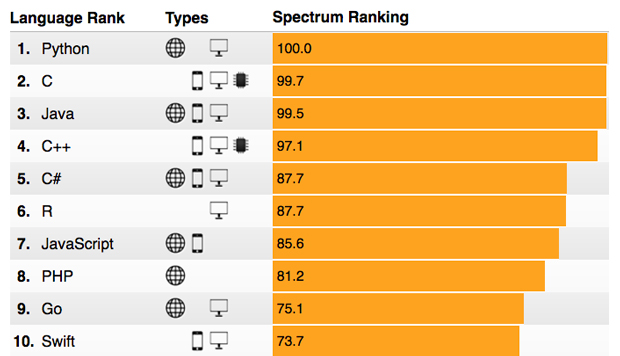
\includegraphics[scale = 0.4]{img/r_ranking_I3E.jpeg}
 \end{center}
\end{figure}

No tópico Ciência de Dados, R e Python são os mais utilizados. É difícil definir 
qual linguagem é melhor neste ponto, havendo diversos sites comparando-as.

Meu objetivo com a linguagem R é contribuir com a 
comunidade gerando conteúdo sobre Arduíno utilizando R, além de contribuir com 
abordagens de análise de dados para a comunidade do Arduino.

Por quê utilizar o Arduíno? 
\begin{citacao}[english]
  "When you start monitoring the environment,
  something happens: You start to understand the world around you in a new way." \cite{Gertz2012}
\end{citacao}

O baixo custo das plataformas de prototipagem, como Arduíno, a 
grande comunidade geradora de conhecimento e a filosofia \emph{open source}
possibilitam a qualquer pessoa, com pouco conhecimento em eletrônica, a
montar sistemas de medições de variáveis ambientais apenas seguindo exemplos 
disponíveis na internet. É possível encontrar: sistemas que medem umidade do 
solo, luminosidade de determinado local, turbidez, condutividade e ph da água, ruídos 
ambientais, e diversas outras variáveis, bastando ter apenas os sensores 
específicos. O Arduíno apresenta baixa complexidade, inclusive há escolas que o utilizam 
para ensino de eletrônica, robótica e programação no ensino médio.
 
Apesar de haver soluções simples\footnote{\url{https://magesblog.com/post/2015-02-17-reading-arduino-data-directly-into-r/}}
para o problema proposto, cabe a esta pesquisa adicionar mais elementos 
referente ao processo de análise de dados, além de fundamentação teórica nas 
etapas, tendo a linguagem de programação R como automatizadora do processo.
\chapter[Justificativa]{Justificativa}


Na comunidade R, existem poucas publicações com relação ao tema proposto. As existentes, são de carater mais 
específico\footnote{\url{https://www.r-bloggers.com/displaying-spatial-sensor-data-from-arduino-with-r-o
n-google-maps/}} veículada em páginas pessoais ou fóruns. 

Neste projeto, abordaremos as partes que compõe a leitura, tratamento e 
apresentação de dados, temas mais comuns aos usuários de R. Serão tratados 
pontos como leitura de dados de um dispositivo de prototipagem (usaremos o 
Arduino), métodos de limpeza e apresentação dos dados, sendo o primeiro por 
algoritmos ou análise dos dados e o segundo por meio de gráficos, planilhas e 
programação literária\footnote{\url{https://en.wikipedia.org/wiki/Literate_programming}}.

Seguindo o paradigma da ciência moderna, este projeto será todo conduzido em 
licença aberta, utilizaremos apenas softwares e hardwares livres, além dos dados 
gerados, análises e scripts implementados estarem disponíveis em repositórios 
abertos como GitHub\footnote{\url{https://github.com/}} e Figshare\footnote{\url{https://figshare.com/}}.

Ao término deste projeto, pretendo alimentar mais discussões envolvendo o R e o 
Arduíno, fazendo com que ambos possam ser aprendidos de forma conjunta e 
difundida. 

\begin{citacao}[english]
  "The modern academic scientist develops code in the open, publishes data and 
code open source, posts preprints of their academic work, still submits to 
traditional journals, and reviews for those journals, but may also write blog 
posts or use social media to critique published work in post-publication review 
fora."\cite{Peng2015}
\end{citacao}


\chapter[Objetivos]{Objetivos}

\section{Objetivo Geral}\label{sec-objetivoGeral}

Desenvolver métodos para obtenção, limpeza e apresentação de dados gerados por 
um dispositivo de prototipagem, utilizando a linguagem de programaçao R e o 
\emph{hardware open source} Arduíno.

\section{Objetivo Específico}\label{sec-objetivoEspecifico}

\begin{alineas}
  
  \item Identificar pacotes do R que permitam interação com interfaces de hardware.
  \item Descrever as formas de comunicação e obtenção de dados entre o R e o hardware.
  \item Sugerir melhorias nos pacotes de comunicação serial.
  \item Aplicar conceitos de limpeza de dados aos dados lidos.
  \item Avaliar técnicas existentes de organização e limpeza de dados.
  \item Identificar pacotes do R que permitam apresentar dados de forma dinâmica e 
  possivelmente em tempo real.
  \item Aplicar métodos de apresentação e resumo de dados.
  \item Implementar um servidor web para visualização dos dados em tempo real.
  
\end{alineas}
\chapter[Referencial Teórico]{Referencial Teórico}

Nosso referencial teórico sobre a linguagem de programação R e análise de dados 
será baseada nas produções acadêmicas de \citeauthoronline{Leek2016}, \citeauthoronline{Peng2015} e 
\citeauthoronline{Caffo2015}. Os autores abordam os passos de um processo de análise de dados e 
suas respectivas ferramentas. Roger Peng em seu livro \emph{R Programming for Data 
Science}\footnote{\url{https://leanpub.com/modernscientist}}  traz os conceitos básicos para a utilização do R como linguagem de 
programação, este livro pode ser considerado um pré-requisito para a leitura dos 
livros seguintes e servirá como base para questões que envolvem programação 
estruturada. Em \emph{Exploratory Data Analysis with R}\footnote{\url{https://leanpub.com/exdata}}, Peng apresenta ferramentas 
em R que são utilizadas na análise exploratória de dados. Neste livro é 
apresentado os pacotes \emph{dplyr} e \emph{ggplot2} para manipulação e apresentação de 
dados. Além disso são apresentadas técnicas de análise, organização e limpeza de 
dados como Hierarchical Clustering, K-Means Clustering e Dimension Reduction. 
Além destas citadas, nesta pesquisa exploraremos outras técnicas de limpeza de 
dados, como as utilizadas em Mineração de Dados.

\begin{citacao}[english]
  "The modern academic scientist develops code in the open, publishes data and 
code open source, posts preprints of their academic work, still submits to 
traditional journals, and reviews for those journals, but may also write blog 
posts or use social media to critique published work in post-publication review 
fora."\cite{Peng2015}
\end{citacao}

\chapter[Metodologia]{Metodologia}

O projeto será iniciado com uma pesquisa sobre os métodos disponíveis em R para 
leitura de dados de um Arduíno. Inicialmente se tem conhecimento do pacote 
\emph{serial} \cite{Seilmayer2017} que fornece métodos para comunicação com uma porta serial. Em seguida, 
utilizando um projeto pronto de Arduíno, iremos efetuar leituras de dados e 
aplicar as técnicas de limpeza de dados. 

Para os pacotes que serão utilizados na manipulação e apresentação de dados, 
\emph{dplyr} e \emph{ggplot2} respectivamente, será efetuado uma pesquisa para 
entendimento completo das funções fornecidas e posteriormente sua aplicação no 
projeto. Este é um dos pontos chaves do projeto já que aqui definiremos ou 
criaremos funções que ficarão em execução enquanto os dados estiverem sendo 
gerados.

Após definido os métodos de leitura, limpeza e apresentação dos dados, será 
iniciado uma pesquisa sobre ferramentas de aplicação \emph{web} que permitam a 
integração da linguagem R. Em seguida iremos montar um servidor web que recebe e 
apresenta em tempo real os dados gerados pelo Arduíno. Para isso, fará parte do 
conhecimento adquirido nesta pesquisa as tecnologias que permitem a criação, 
hospedagem e modelagem de um servidor de aplicação \emph{web}.

Ao final do projeto, pretende-se apresentar um sistema que mostre em tempo real, 
informações (gráficos, tabelas, resumos) de dados gerados por um dispositivo de 
prototipagem Arduíno.
\chapter[Cronograma]{Cronograma}

Este pesquisa será realizada em 7 meses, conforme \autoref{tabCrono}, tendo três importantes divisões. Na 
primeira parte, será concentrada a pesquisa sobre o tema e o aperfeiçoamento 
técnico nas ferramentas de R e Arduino.

Na segunda parte aplicarei os resultados gerados nos pontos anteriores em um 
sistema web, que será desenvolvido como parte deste projeto.

Por último, a compilação dos resultados serão transcritos no relatório final de 
iniciação científica.

\begin{table}[htb]
  \centering
  \caption[Cronograma]{Cronograma}
  \label{tabCrono}
  \begin{tabular}{llllllll}
    \textbf{Atividades}                    		& \textbf{Jun} & \textbf{Jul} & \textbf{Ago} & \textbf{Set} & \textbf{Out} & \textbf{Nov} & \textbf{Dez} \\
    \hline
    Pesquisa Bibliográfica                 		& X   & X   & X   & X   & X   & X   & X   \\
    Estudo de métodos de comunicação em R  		& X   &     &     &     &     &     &     \\
    Relatórios bimestrais                  		& X   &     & X   &     & X   &     & X   \\
    Estudo dos pacotes \emph{dplyr} e \emph{ggplot2} 	&     & X   & X   &     &     &     &     \\
    Pesquisa sobre técnicas de limpeza de dados 	&     & X   & X   & X   & X   & X   &     \\
    Desenvolvimento do script R 			&     & X   & X   & X   & X   & X   & X   \\
    Pesquisa sobre aplicações web 			&     &     &     &     &     & X   & X   \\
    Desenvolvimento aplicação web 			&     &     &     &     &     & X   & X   \\
    Elaboração e revisão da monografia 			&     &     &     &     &     &     & X   \\
    Elaboração e revisão do artigo científico 		&     &     &     &     &     &     & X   \\
    \hline
  \end{tabular}
\end{table}



% ---
% Finaliza a parte no bookmark do PDF
% para que se inicie o bookmark na raiz
% e adiciona espaço de parte no Sumário
% ---
\phantompart

% ---
% Conclusão
% ---
\chapter*[Considerações finais]{Considerações finais}
\addcontentsline{toc}{chapter}{Considerações finais}

\lipsum[31-33]

% ----------------------------------------------------------
% ELEMENTOS PÓS-TEXTUAIS
% ----------------------------------------------------------
\postextual

% ----------------------------------------------------------
% Referências bibliográficas
% ----------------------------------------------------------
\bibliography{refs/refs.bib}

% ----------------------------------------------------------
% Glossário
% ----------------------------------------------------------
%
% Consulte o manual da classe abntex2 para orientações sobre o glossário.
%
%\glossary

% ----------------------------------------------------------
% Apêndices
% ----------------------------------------------------------

% ---
% Inicia os apêndices
% ---
\begin{apendicesenv}

% Imprime uma página indicando o início dos apêndices
\partapendices

% ----------------------------------------------------------
\chapter{Quisque libero justo}
% ----------------------------------------------------------

\lipsum[50]

% ----------------------------------------------------------
\chapter{Nullam elementum urna vel imperdiet sodales elit ipsum pharetra ligula
ac pretium ante justo a nulla curabitur tristique arcu eu metus}
% ----------------------------------------------------------
\lipsum[55-57]

\end{apendicesenv}
% ---


% ----------------------------------------------------------
% Anexos
% ----------------------------------------------------------

% ---
% Inicia os anexos
% ---
\begin{anexosenv}

% Imprime uma página indicando o início dos anexos
\partanexos

% ---
\chapter{Morbi ultrices rutrum lorem.}
% ---
\lipsum[30]

% ---
\chapter{Cras non urna sed feugiat cum sociis natoque penatibus et magnis dis
parturient montes nascetur ridiculus mus}
% ---

\lipsum[31]

% ---
\chapter{Fusce facilisis lacinia dui}
% ---

\lipsum[32]

\end{anexosenv}

%---------------------------------------------------------------------
% INDICE REMISSIVO
%---------------------------------------------------------------------

\phantompart

\printindex


\end{document}
